\documentclass[12pt]{article}
\usepackage{geometry}
\geometry{margin=1in}
\usepackage{tikz}
\usetikzlibrary{arrows.meta, positioning}

\title{File Management System}
\author{Lizbeth Ochoa}
\date{}

\begin{document}
\maketitle

\section{Introduction}
P3: File System Implementation is an implementation of a file management system that shows operating systems file handling concepts. The application allows CRUD operations as well as rename and navigate on files and directories.

I chose Python in this project because of my familiarity with the language and how simple it is. As well as how it supports file operations through the os module. Paired with Tkinter as recommended for GUI development because of how well it integrates with Python.

\section{Operating System Concepts}
The application uses system level file operation like open(), read(), write(), close(), and rename() on the OS module.

File descriptors are then used internally by the OS when files are being opened. The application uses Python's "with open" to ensure proper allocation and release of the file descriptors.

Metadata is retrieved and stored by Inodes. Such as permissions and file size, and directory entries map filenames to inode numbers.

\section{Design and Architecture}

\begin{center}
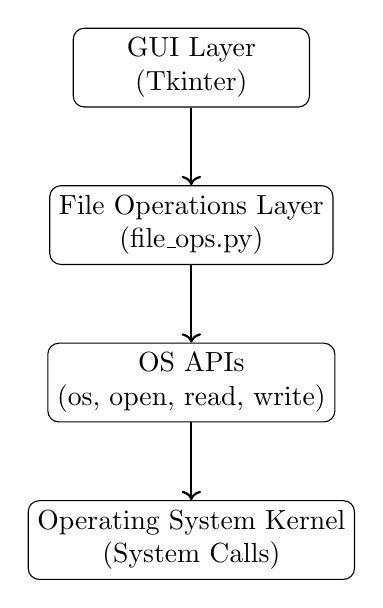
\begin{tikzpicture}[
    node distance=2cm,
    every node/.style={draw, rectangle, rounded corners, align=center, minimum width=3cm, minimum height=1cm},
    arrow/.style={->, thick}
]

\node (gui) {GUI Layer \\ (Tkinter)};
\node (ops) [below of=gui] {File Operations Layer \\ (file\_ops.py)};
\node (os) [below of=ops] {OS APIs \\ (os, open, read, write)};
\node (kernel) [below of=os] {Operating System Kernel \\ (System Calls)};

\draw[arrow] (gui) -- (ops);
\draw[arrow] (ops) -- (os);
\draw[arrow] (os) -- (kernel);

\end{tikzpicture}
\end{center}

\end{document}
